\chapter{Methodology}

 % Replace with your text


\section{Requirements}


In order to run the project, there are some requirements:
\begin{itemize}
\item A working Java 8 or 11 installation.
\item Have the flinkmancer.jar .  
\item Download Apache Flink 1.10.1 for Scala 2.12
\end{itemize}
After the downloaded archive is unpacked, flink has to be configured for the standalone cluster. The "/conf" directory has 2 important files.
\begin{itemize}
\item flink-conf.yaml:

In this file we set: 
\newline "jobmanager.rpc.address"  to be the IP of Job Manager. 
\newline "taskmanager.memory.flink.size" to be the highest available DRAM. 
\newline "taskmanager.memory.off-heap.size" to at least 1024m. 
\newline "taskmanager.numberOfTaskSlots" to the number of cores each machine has. 
\newline "taskmanager.memory.network.min" and "taskmanager.memory.network.max" 
\newline in a way that flink.size * network.fraction (0.1) is between min and max.

\item slaves:

In this file we add the id of each machine that will run a task manager. 
\end{itemize}
Now we can start our cluster and run the project
\begin{itemize}
\item  “ ./flink-1.10.0/bin/start-cluster.sh “ 
\item  “ ./flink-1.10.0/bin/flink run flinkmancer.jar -{}-cores [number of total cores] -{}-path [path to dataset] -{}-outpath [path to output file inclunding the name]“ 
\end{itemize}

The data sets needs to be in ./data/{layer} for each different layer used. \newline 
In our test runs we used 4 different layers, “follow”, ”reply”, ”quote”, ”retweet”.
After the program is executed , it produces a Features.csv file, containing 100 Features about each Edge of Vectors (each Vector being a user) and their common neighbors. 




\section{Design}
We wanted to create a Dataset of every node paired with a list of every neighbor for every layer examined in the process. We achieved that, by reading each layer's data, creating 2 adjacent lists for every layer, one for incoming neighbors and one for outgoing. Then we used outer join to combine them and have an 'empty' slot for every missing link. The reason to go for full outer join is we want to keep any neighbor and not only the common neighbors at incoming and outgoing.

For example: Imagine we have Node 1 , with incoming Nodes 2,3 and outgoing 3,4. What outer join does for us is that our result is a Tuple of 2 lists ([2,3,[]],[[],3,4]) instead of ([3][3]).

We use the same technique for every Tuple we created on the previous step and we combine them in a final Tuple of 8 lists (4 layers in this process).  Now we have a Dataset that contains a Tuple of (Id,Tuple8(8 lists of neighbors, 2 for each layer)). 
We transformed this Dataset of Tuples into Dataset of "Nodes". Node is a POJO with 2 variables: 
\begin{itemize}
    \item Long Id
    \item ArrayList \textless Set\textless Long\textgreater \textgreater  Sets
\end{itemize}

We create a cross product of this Dataset with itself. This will create every possible edge given our known ids. The result was a Dataset of (Node,Node) . We applied function Feat() to each pair of nodes using flatMap , and got the result containing all features. The Feat() function creates an Array where it stores every feature. It later creates a string of comma-separated values that starts with the Id of U - V and continues with the features.  The algorithm of selecting features is explained in detail here[1] and here[3]. 

In our tests we have a total of 100 features for each Edge, so we produce an output of 102 numbers (2 node ides and 100 features). The diagram of our project is shown in Figure 1.

The alternative method we used to reduce the output size, essentially takes the result of Feat() and calculates the length of each line. The new output is irrelevant but it allows to lower the size by a factor of 100 since we now have only 2 Long per line instead of 102.



\section{Implementation}

This is a Maven Project written in Java using Apache Flink. 

It contains 3 .java files:
\begin{itemize} 
\item Flinkmancer.java
\item Features.java
\item Node.java
\end{itemize}

Flinkmancer.java is main class of the project. It sets up the flink environment, reads the data input for each layer and creates the adjacent lists of neighbors which then combines using outer join function. These lists are transformed into Nodes. Those nodes are then used to create a cross product with themselves. using .cross function provided by flink, and stored in a Dataset. we apply a Feat() function to every edge in our cross product and we receive a final Tuple of 2, (ids,features). \newline

Node.java is simply the class that implements the Node objects, and contains ways to access each object variables such us setId(), getId(), getSets() as well as the class constructors. \newline

Features.java contains the feature extraction function Feat(). This function uses the Dataset of all Nodes created in Flinkmancer.java to extract 100 features for each Node Edge. It returns an array of 102 columns, first 2 being the ID of nodes , and rest 100 the features in form of Tuple2 .
\begin{figure}[ht]
\noindent\makebox[\textwidth]{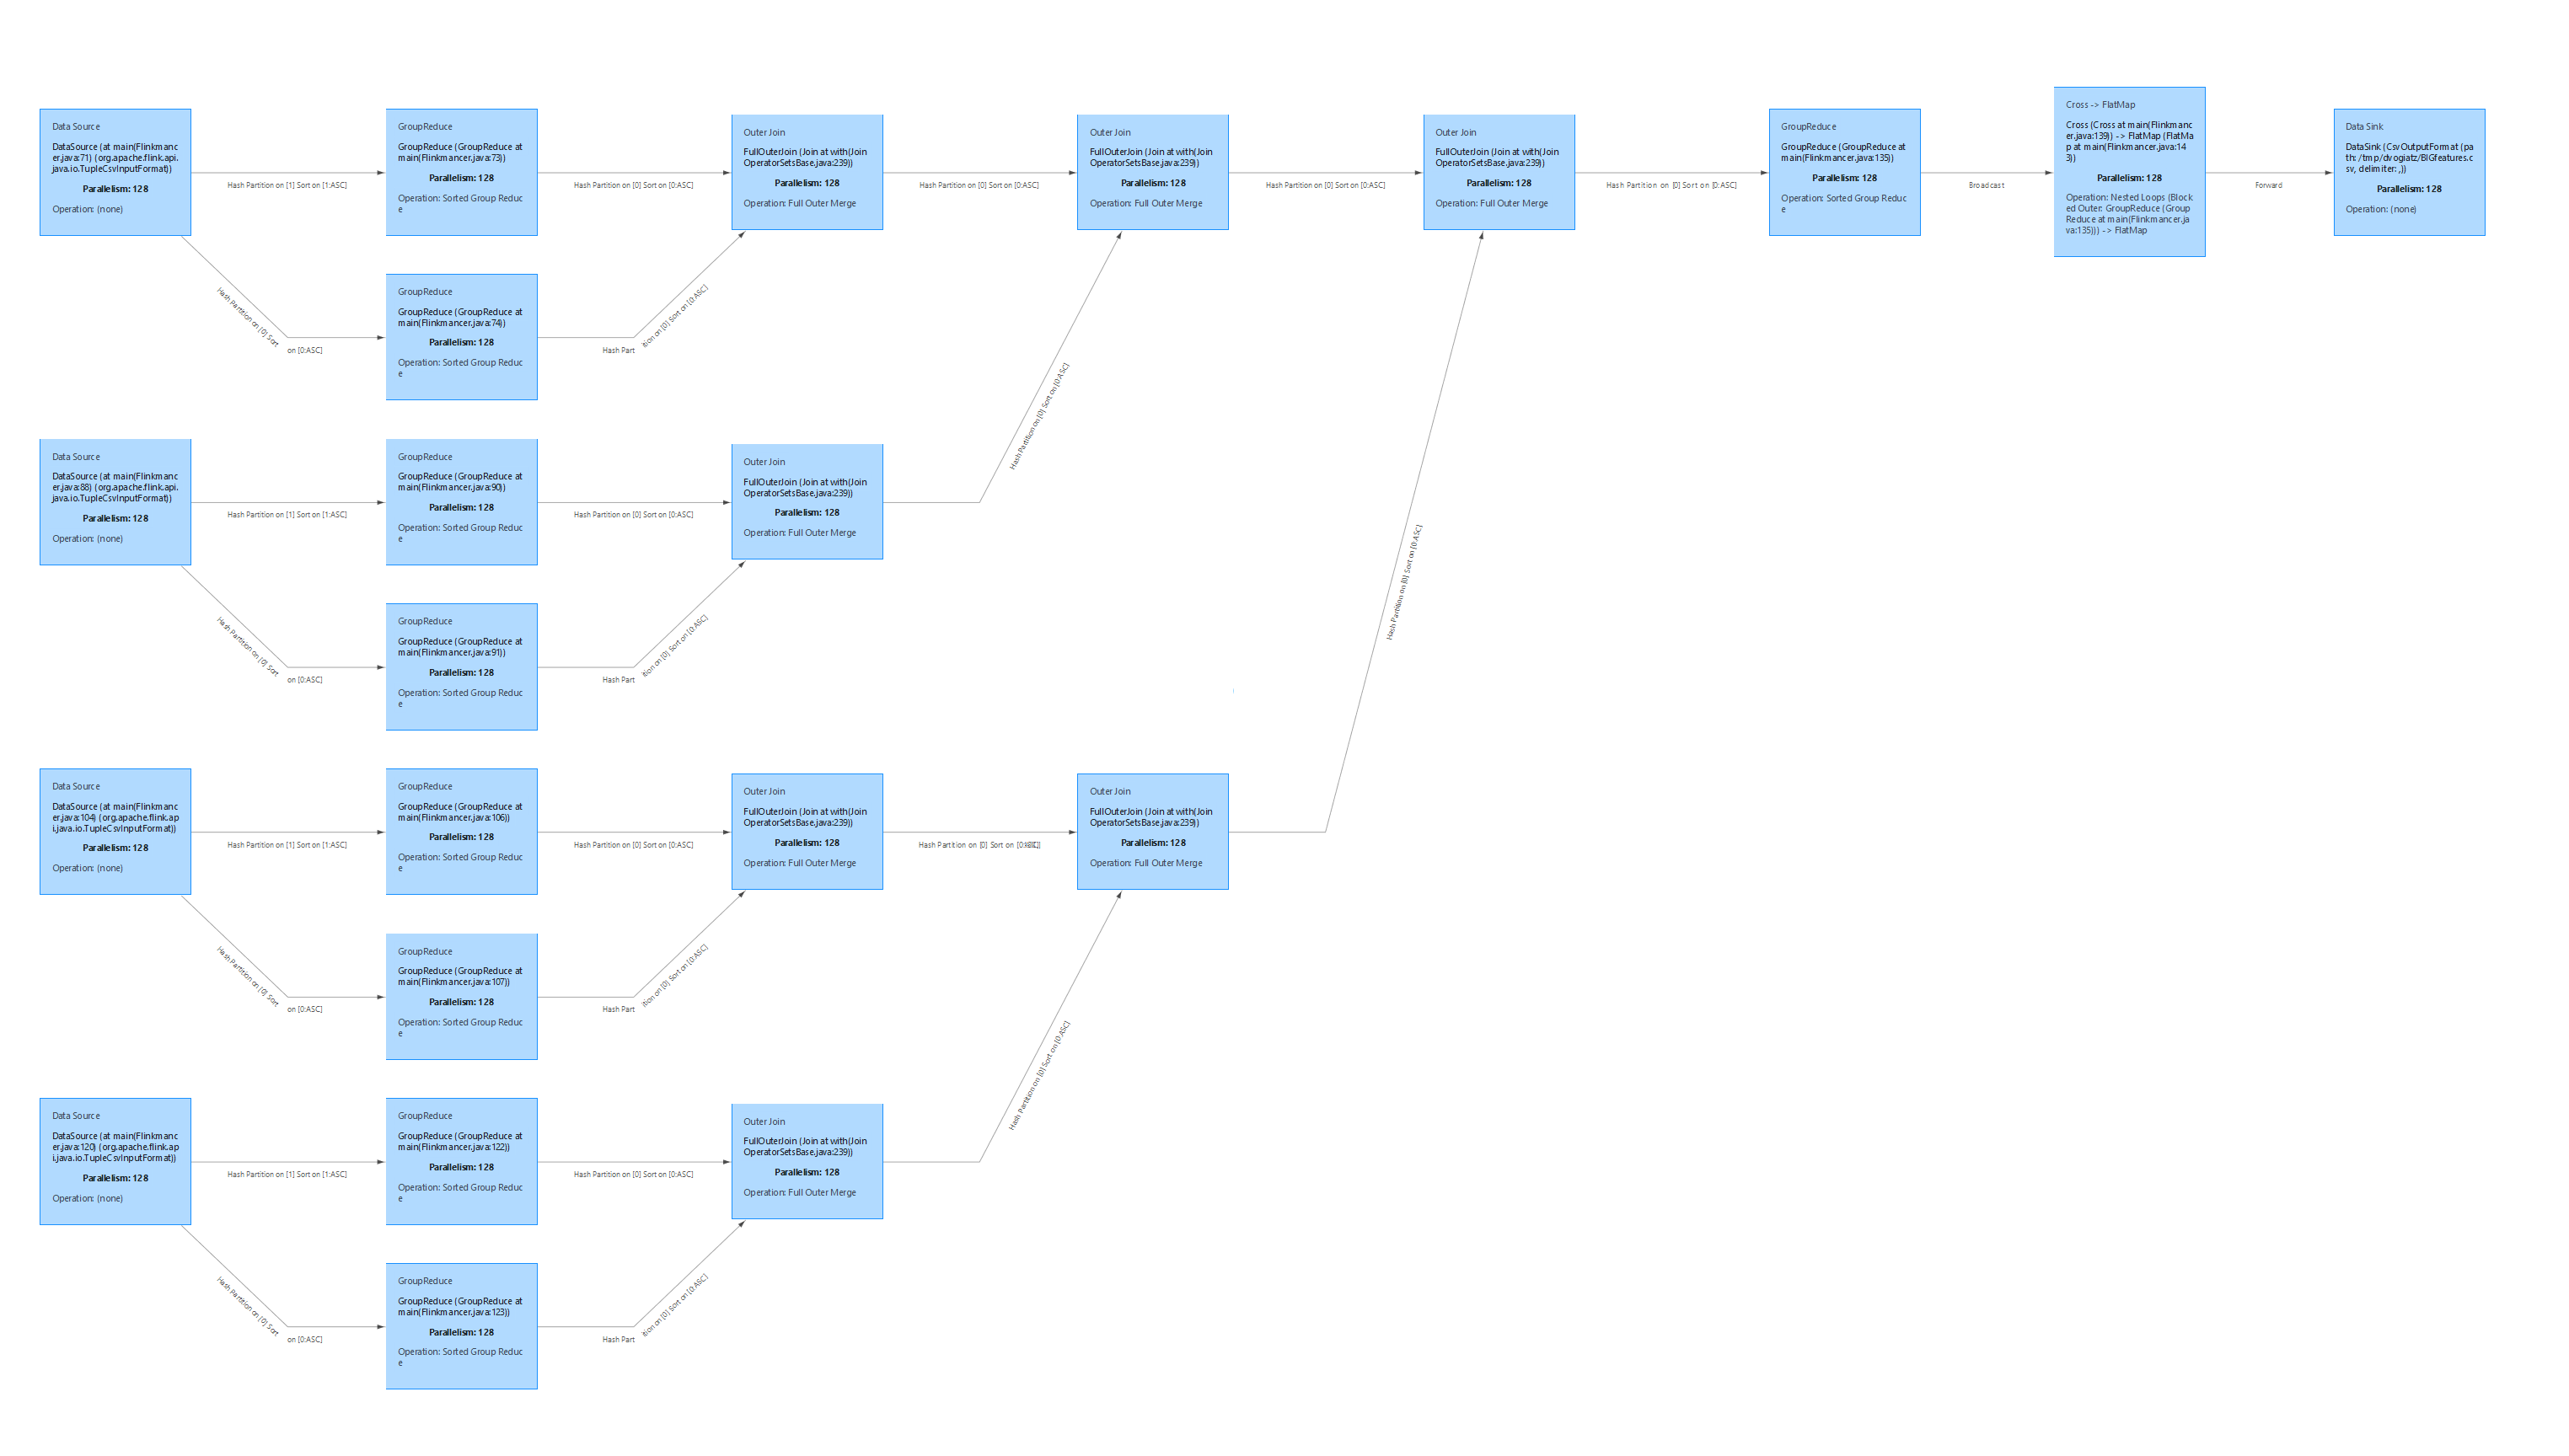
\includegraphics[width=\textwidth]{Thesis/images/diagram.png}}
\caption{Every process that takes place in the project}
\label{fig:graph}
\end{figure}
